\documentclass{standalone}
\usepackage{tikz}
\usetikzlibrary{patterns, positioning}
\usepackage[sfdefault]{ClearSans} %% option 'sfdefault' activates Clear Sans as the default text font
\usepackage[T1]{fontenc}

\begin{document}
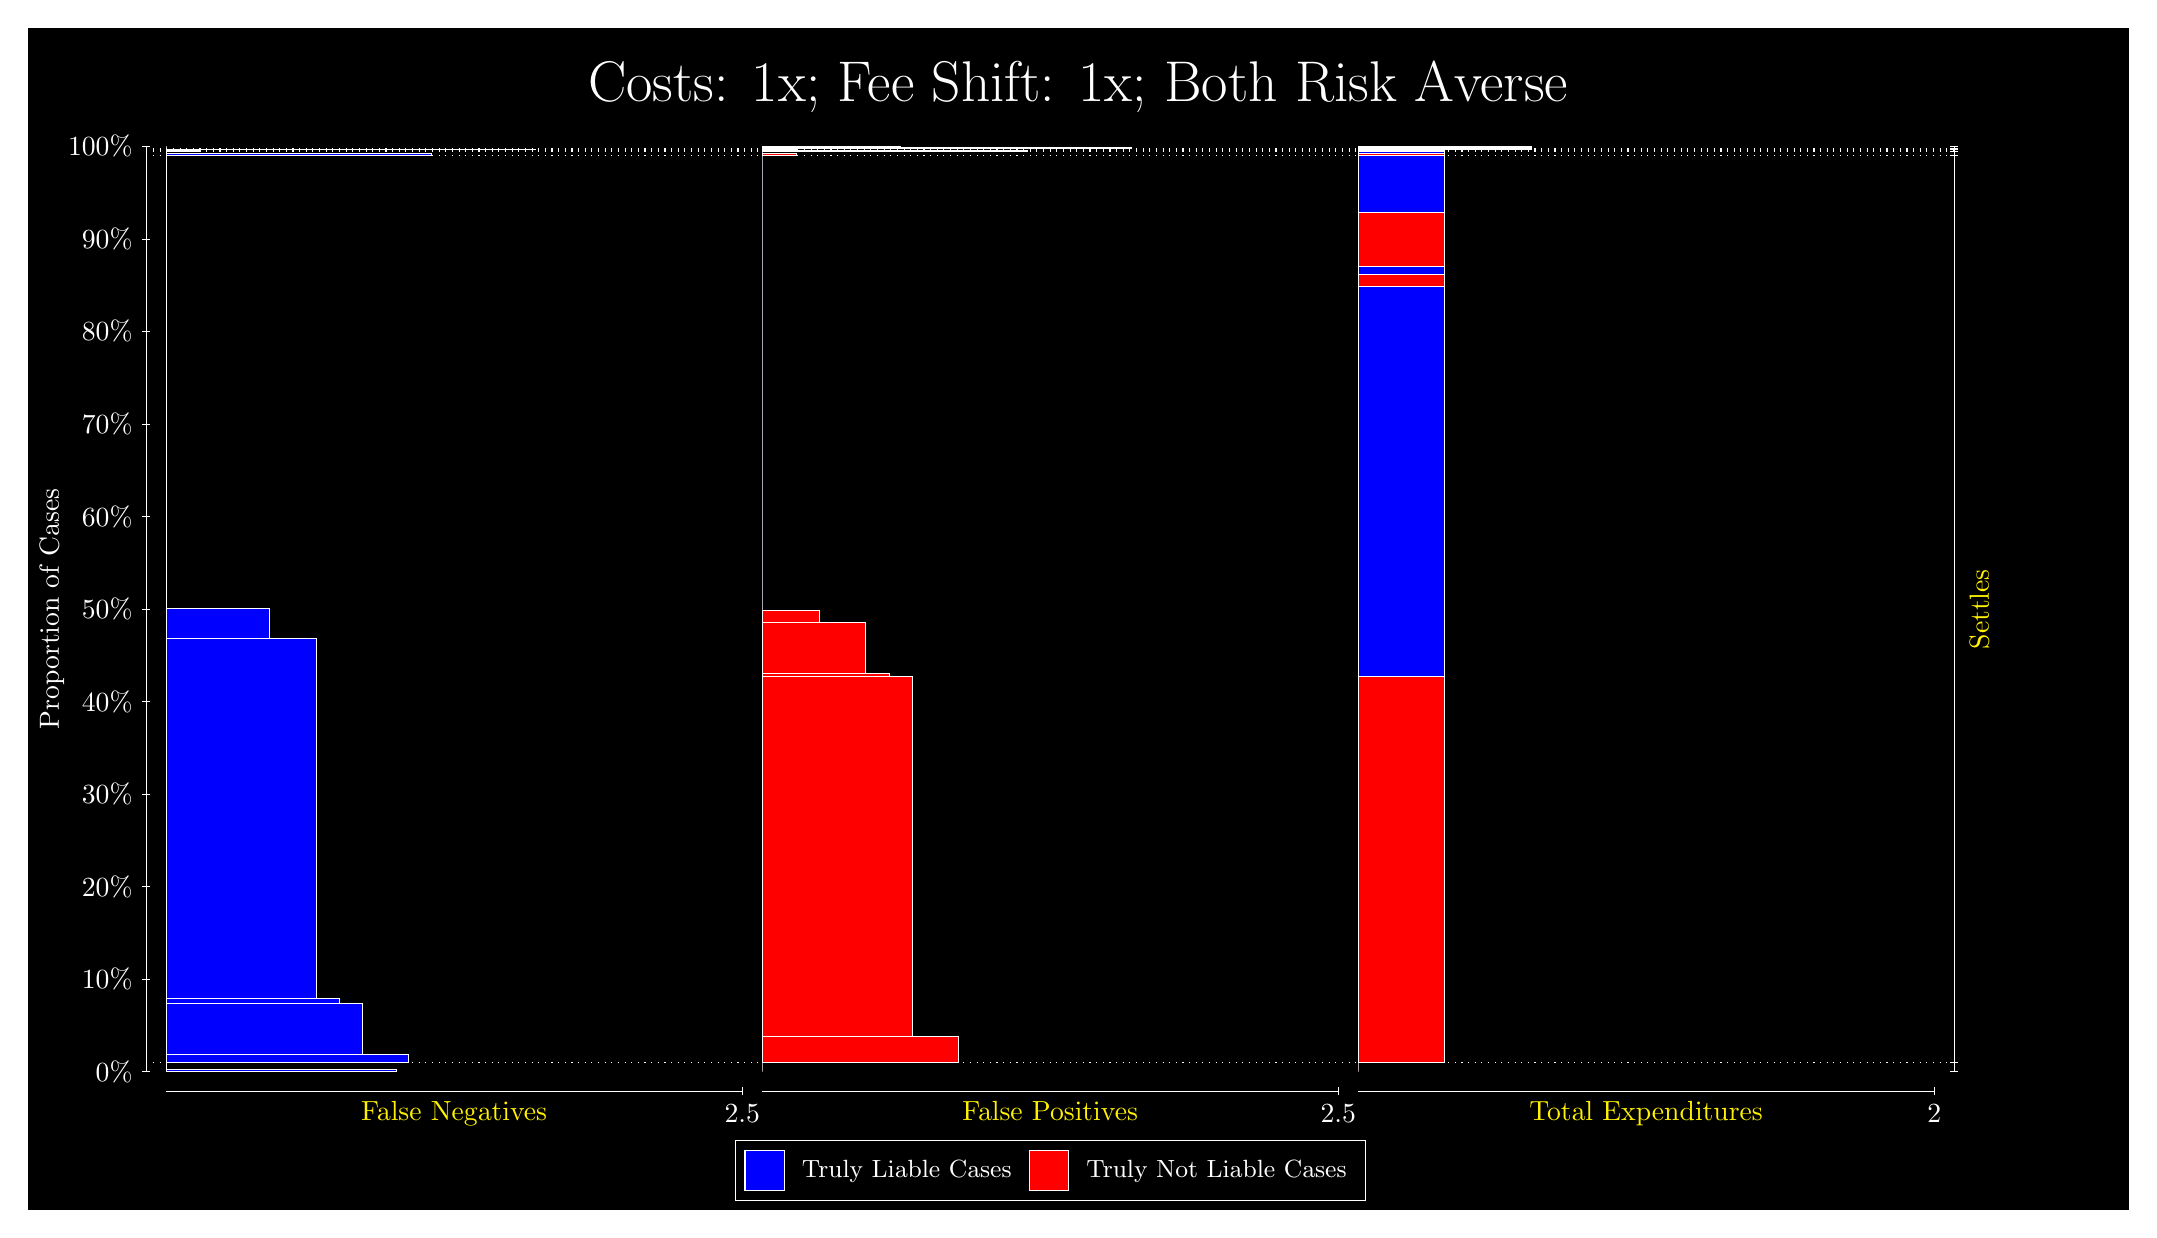
\begin{tikzpicture}
\draw[fill=black] (0,0) rectangle (26.667,15);
\draw[text=white] (0,13.5) rectangle (26.667,15) node[midway] {\huge Costs: 1x; Fee Shift: 1x; Both Risk Averse};
\draw[white, very thin] (1.5,1.75) -- (1.5,13.5);
\node[rotate=90, text=white, anchor=center] at (0.3, 7.625) {Proportion of Cases};
\draw[white, very thin] (1.45,1.75) -- (1.55,1.75);
\node[text=white, anchor=east] at (1.45, 1.75) {0\%};
\draw[white, very thin] (1.45,2.925) -- (1.55,2.925);
\node[text=white, anchor=east] at (1.45, 2.925) {10\%};
\draw[white, very thin] (1.45,4.1) -- (1.55,4.1);
\node[text=white, anchor=east] at (1.45, 4.1) {20\%};
\draw[white, very thin] (1.45,5.275) -- (1.55,5.275);
\node[text=white, anchor=east] at (1.45, 5.275) {30\%};
\draw[white, very thin] (1.45,6.45) -- (1.55,6.45);
\node[text=white, anchor=east] at (1.45, 6.45) {40\%};
\draw[white, very thin] (1.45,7.625) -- (1.55,7.625);
\node[text=white, anchor=east] at (1.45, 7.625) {50\%};
\draw[white, very thin] (1.45,8.8) -- (1.55,8.8);
\node[text=white, anchor=east] at (1.45, 8.8) {60\%};
\draw[white, very thin] (1.45,9.975) -- (1.55,9.975);
\node[text=white, anchor=east] at (1.45, 9.975) {70\%};
\draw[white, very thin] (1.45,11.15) -- (1.55,11.15);
\node[text=white, anchor=east] at (1.45, 11.15) {80\%};
\draw[white, very thin] (1.45,12.325) -- (1.55,12.325);
\node[text=white, anchor=east] at (1.45, 12.325) {90\%};
\draw[white, very thin] (1.45,13.5) -- (1.55,13.5);
\node[text=white, anchor=east] at (1.45, 13.5) {100\%};

\draw[white, very thin] (24.457,1.75) -- (24.457,13.5);
\draw[white, very thin] (24.407,1.75) -- (24.507,1.75);
\node[anchor=west] at (24.407, 1.75) {};
\draw[white, very thin] (24.407,1.8641) -- (24.507,1.8641);
\node[anchor=west] at (24.407, 1.8641) {};
\draw[white, very thin] (24.407,13.38) -- (24.507,13.38);
\node[anchor=west] at (24.407, 13.38) {};
\draw[white, very thin] (24.407,13.441) -- (24.507,13.441);
\node[anchor=west] at (24.407, 13.441) {};
\draw[white, very thin] (24.407,13.459) -- (24.507,13.459);
\node[anchor=west] at (24.407, 13.459) {};
\draw[white, very thin] (24.407,13.477) -- (24.507,13.477);
\node[anchor=west] at (24.407, 13.477) {};
\draw[white, very thin] (24.407,13.5) -- (24.507,13.5);
\node[anchor=west] at (24.407, 13.5) {};

\draw[white, very thin, fill=blue] (1.75,1.75) rectangle (4.6775,1.7813);
\draw[white, very thin, fill=red] (1.75,1.7813) rectangle (1.75,1.8641);
\draw[white, very thin, fill=blue] (1.75,1.8641) rectangle (4.8239,1.969);
\draw[white, very thin, fill=blue] (1.75,1.969) rectangle (4.2384,2.6218);
\draw[white, very thin, fill=blue] (1.75,2.6218) rectangle (3.9457,2.685);
\draw[white, very thin, fill=blue] (1.75,2.685) rectangle (3.6529,7.2545);
\draw[white, very thin, fill=blue] (1.75,7.2545) rectangle (3.0674,7.6335);
\draw[white, very thin, fill=red] (1.75,7.6335) rectangle (1.75,13.38);
\draw[white, very thin, fill=blue] (1.75,13.38) rectangle (5.1167,13.415);
\draw[white, very thin, fill=red] (1.75,13.415) rectangle (1.75,13.441);
\draw[white, very thin, fill=blue] (1.75,13.441) rectangle (2.1891,13.455);
\draw[white, very thin, fill=red] (1.75,13.455) rectangle (1.75,13.459);
\draw[white, very thin, fill=blue] (1.75,13.459) rectangle (6.4341,13.468);
\draw[white, very thin, fill=red] (1.75,13.468) rectangle (1.75,13.477);
\draw[white, very thin, fill=red] (1.75,13.477) rectangle (1.75,13.483);
\draw[white, very thin, fill=blue] (1.75,13.483) rectangle (1.75,13.5);
\draw[white, very thin, fill=red] (9.3189,1.75) rectangle (9.3189,1.8328);
\draw[white, very thin, fill=blue] (9.3189,1.8328) rectangle (9.3189,1.8641);
\draw[white, very thin, fill=red] (9.3189,1.8641) rectangle (11.807,2.2033);
\draw[white, very thin, fill=red] (9.3189,2.2033) rectangle (11.222,6.7728);
\draw[white, very thin, fill=red] (9.3189,6.7728) rectangle (10.929,6.8052);
\draw[white, very thin, fill=red] (9.3189,6.8052) rectangle (10.636,7.458);
\draw[white, very thin, fill=red] (9.3189,7.458) rectangle (10.051,7.611);
\draw[white, very thin, fill=blue] (9.3189,7.611) rectangle (9.3189,13.38);
\draw[white, very thin, fill=red] (9.3189,13.38) rectangle (9.758,13.406);
\draw[white, very thin, fill=blue] (9.3189,13.406) rectangle (9.3189,13.441);
\draw[white, very thin, fill=red] (9.3189,13.441) rectangle (12.686,13.445);
\draw[white, very thin, fill=blue] (9.3189,13.445) rectangle (9.758,13.459);
\draw[white, very thin, fill=red] (9.3189,13.459) rectangle (9.3189,13.468);
\draw[white, very thin, fill=blue] (9.3189,13.468) rectangle (9.3189,13.477);
\draw[white, very thin, fill=red] (9.3189,13.477) rectangle (14.003,13.483);
\draw[white, very thin, fill=blue] (9.3189,13.483) rectangle (11.075,13.5);
\draw[white, very thin, fill=red] (16.888,1.75) rectangle (16.888,1.8328);
\draw[white, very thin, fill=blue] (16.888,1.8328) rectangle (16.888,1.8641);
\draw[white, very thin, fill=red] (16.888,1.8641) rectangle (17.986,6.7728);
\draw[white, very thin, fill=blue] (16.888,6.7728) rectangle (17.986,11.721);
\draw[white, very thin, fill=red] (16.888,11.721) rectangle (17.986,11.874);
\draw[white, very thin, fill=blue] (16.888,11.874) rectangle (17.986,11.979);
\draw[white, very thin, fill=red] (16.888,11.979) rectangle (17.986,12.664);
\draw[white, very thin, fill=blue] (16.888,12.664) rectangle (17.986,13.38);
\draw[white, very thin, fill=red] (16.888,13.38) rectangle (17.986,13.406);
\draw[white, very thin, fill=blue] (16.888,13.406) rectangle (17.986,13.441);
\draw[white, very thin, fill=red] (16.888,13.441) rectangle (17.986,13.445);
\draw[white, very thin, fill=blue] (16.888,13.445) rectangle (17.986,13.459);
\draw[white, very thin, fill=red] (16.888,13.459) rectangle (19.083,13.468);
\draw[white, very thin, fill=blue] (16.888,13.468) rectangle (19.083,13.477);
\draw[white, very thin, fill=red] (16.888,13.477) rectangle (19.083,13.483);
\draw[white, very thin, fill=blue] (16.888,13.483) rectangle (19.083,13.5);
\draw[white, dotted] (1.5,1.8641) -- (24.457,1.8641);
\draw[white, dotted] (1.5,13.38) -- (24.457,13.38);
\draw[white, dotted] (1.5,13.441) -- (24.457,13.441);
\draw[white, dotted] (1.5,13.459) -- (24.457,13.459);
\draw[white, dotted] (1.5,13.477) -- (24.457,13.477);
\draw[white, very thin] (1.75,1.5) -- (9.0689,1.5);
\node[text=yellow, anchor=north] at (5.4094, 1.5) {False Negatives};
\draw[white, very thin] (9.0689,1.45) -- (9.0689,1.55);
\node[text=white, anchor=north] at (9.0689, 1.45) {2.5};

\draw[white, very thin] (9.3189,1.5) -- (16.638,1.5);
\node[text=yellow, anchor=north] at (12.978, 1.5) {False Positives};
\draw[white, very thin] (16.638,1.45) -- (16.638,1.55);
\node[text=white, anchor=north] at (16.638, 1.45) {2.5};

\draw[white, very thin] (16.888,1.5) -- (24.207,1.5);
\node[text=yellow, anchor=north] at (20.547, 1.5) {Total Expenditures};
\draw[white, very thin] (24.207,1.45) -- (24.207,1.55);
\node[text=white, anchor=north] at (24.207, 1.45) {2};


\node[text=yellow, centered, rotate=90] at (24.777, 7.6222) {Settles};





\draw (12.978300999999998,1.5) node[draw=none] (baseCoordinate) {};
\begin{scope}[align=center]
        \matrix[scale=0.5, draw=white, below=0.5cm of baseCoordinate, nodes={draw}, column sep=0.1cm]{
            \node[rectangle, draw, minimum width=0.5cm, minimum height=0.5cm, fill=blue] {}; &
            \node[draw=none, font=\small, text=white] (B) {Truly Liable Cases}; &
            \node[rectangle, draw, minimum width=0.5cm, minimum height=0.5cm, fill=red] {}; &
            \node[draw=none, font=\small, text=white] (B) {Truly Not Liable Cases}; \\
            };
\end{scope}

\end{tikzpicture}
\end{document}